\documentclass[a4paper, 12pt]{article}
\usepackage[T2A]{fontenc}
\usepackage[utf8]{inputenc}
\usepackage[russian]{babel}
\usepackage{amsmath}
\usepackage{indentfirst}
\usepackage{graphicx}
\usepackage[top=2cm, bottom=2cm, left=3cm, right=1cm]{geometry}

\newcommand{\Pra}{\mathbf{Pr}}
\newcommand{\Gra}{\mathbf{Gr}}
\newcommand{\der}[2]{\frac{\partial {#1}}{\partial {#2}}}
\newcommand{\dder}[2]{\frac{\partial^2 {#1}}{\partial {#2}^2}}
\newcommand{\psp}[2]{\psi_{\mathring{#1}}^{#2}}

\begin{document}
  \begin{titlepage}
    \begin{center} %% ПО ЦЕНТРУ
      \bfseries

      {\Large Белорусский государственный университет}

      \vspace{96pt}

      {\large Факультет прикладной математики и информатики}

      \vspace{72pt}

      {\large Кафедра вычислительной математики}

      \vspace{96pt}

      Отчет по лабораторной работе

      \vspace{24pt}

      Вариант №4

      \vspace{24pt}

      {\Large Вычислительный эксперимент в конвекции}

    \end{center}

    \vspace{120pt}

    \begin{flushright}
      \begin{tabular}{rl}
        Подготовили: & Д.\,Г. Борисевич \\
                     & И.\,И. Демух \\
                     & В.\,A. Сидоров \\
                     &студенты 5 курса 5 группы\\
        Преподаватель: & В.\,К. Полевиков \\
      \end{tabular}
    \end{flushright}

    \vfill

    \begin{center}
      \bfseries
      Минск, 2016
    \end{center}
  \end{titlepage}

  \section{Постановка задачи}
    Решить задачу естественной конвекции несжимаемой жидкости в двумерной
    области.
    \begin{itemize}
      \item Монтонная разностная схема порядка $O(h)$
      \item Граничные условия
      \item Параметры: число Прандтля $\Pra=1.0$ и число Грасгофа
        $\Gra=[100;10000]$
    \end{itemize}
  \pagebreak

  \section{Уравнение конвекции}
    При составлении уравнения конвекции будем считать, что жидкость несжимаема и
    в объеме отсутсвуют источники тепла.

    Уравнение гравитационной конвекции с несжимаемой жидкостю и отсутствием
    источников тепла внутри жидкости:

    $$
      \left\{
        \begin{aligned}
          &\der{T}{t} + \der{\psi}{y} \der{T}{x} - \der{\psi}{x} \der{T}{y} =
            a \left( \dder{T}{x} + \dder{T}{y} \right)
          \\
          &\dder{\psi}{x} + \dder{\psi}{y} + \omega = 0
          \\
          &\der{\omega}{t} + \der{\psi}{y} \der{\omega}{x} - \der{\psi}{x}
            \der{\omega}{y} = \nu \left(
              \dder{\omega}{x} + \dder{\omega}{y}
            \right) + \beta g \der{T}{x}
        \end{aligned}
      \right.
    $$

    Безразмерная форма:

    $$
      \left\{
        \begin{aligned}
          &\der{\psi}{y} \der{T}{x} - \der{\psi}{x} \der{T}{y} = \frac{1}{Pr}
            \left( \dder{T}{x} + \dder{T}{y} \right)
          \\
          &\dder{\psi}{x} + \dder{\psi}{y} + \omega = 0
          \\
          &\der{\psi}{y} \der{\omega}{x} - \der{\psi}{x} \der{\psi}{y} =
            \dder{\omega}{x} + \dder{\omega}{y} + Gr \der{T}{x}
        \end{aligned}
      \right.
    $$

    где $Pr = \frac{v}{a}, \quad Gr = \frac{\beta g \Delta T l^{3}}{\nu}$
  \pagebreak

  \section{Разностная схема для уравнений конвекции}
    После введения безразмерных величин, область решения задачи представляет
    собой единичный квадрат. Построим равномерную сетку с длиной шага h по обоим
    направлениям и заменим исходную дифференциальную задачу разностной на
    построенной сетке узлов.

    Введем обозначения:
    \begin{gather*}
      f_{\mathring{x}} = \frac{f_{i+1,j} - f_{i-1,j}}{2 h}
      \\
      f_{\mathring{y}} = \frac{f_{i,j+1} - f_{i,j-1}}{2 h}
      \\
      f_{\overline{x}} = \frac{f_{i,j} - f_{i-1,j}}{h}
      \\
      f_{y} = \frac{f_{i,j+1} - f_{i,j}}{h}
      \\
      f_{x \overline{x}} = \frac{f_{i+1,j} - 2 f_{i,j} + f_{i-1,j}}{h^2}
      \\
      f^{+} = \left\{
        \begin{aligned}
          &f, \quad f > 0\\
          &0, \quad f \leq 0
        \end{aligned}
      \right.
      \\
      f^{-} = \left\{
        \begin{aligned}
          &f, \quad f < 0\\
          &0, \quad f \geq 0
        \end{aligned}
      \right.
    \end{gather*}

    Получим разностную схему:
    \begin{equation}
      \left\{
        \begin{aligned}
          &\left( \psp{y}{+} T_{\overline{x}} + \psp{y}{-} T_{x} \right) -
            \left( \psp{x}{+} T_{y} + \psp{x}{-} T_{\overline{y}} \right) =
            \frac{1}{\Pra}\left( T_{x \overline{x}} + T_{y \overline{y}} \right)
          \\
          &\psi_{x \overline{x}} + \psi_{y \overline{y}} + \omega = 0
          \\
          &\left(
            \psp{y}{+} \omega_{\overline{x}} + \psp{y}{-} \omega_{x}
          \right) - \left(
            \psp{x}{-} \omega_{\overline{y}} + \psp{x}{+} \omega_{y}
          \right) =
            \omega_{x \overline{x}} + \omega_{y \overline{y}} +
            \Gra T_{\mathring{x}}
        \end{aligned}
      \right.\label{diff_scheme}
    \end{equation}

    Каждая из этих трёх разностных схем является монотонной и аппроксимирует
    соответствующее дифференциальное уравнение с первым порядком точности.
    Построим итерационный процесс. Для каждого узла вычислияем значения
    температуры, функций тока и вихря по следующим расчетным формулам, которые
    следуют из \eqref{diff_scheme}:

    \begin{equation}
      \left\{
        \begin{aligned}
          &T_{i,j} =
            \frac{
              T_{i-1,j}\left(
                1 + h \Pra \psp{y}{+}
              \right) +
              T_{i,j-1}\left(
                1 - h \Pra \psp{x}{-}
              \right) +
              T_{i+1,j}\left(
                1 - h \Pra \psp{y}{-}
              \right) +
              T_{i,j+1}\left(
                1 + h \Pra \psp{x}{+}
              \right)
            }{4 + h \Pra \left(
              \psp{y}{+} + \psp{x}{+} - \psp{y}{-} - \psp{x}{-}
            \right)}
          \\
          &\psi_{i,j} = \frac{1}{4} \left(
            \psi_{i,j+1} + \psi_{i,j-1} + \psi_{i-1,j} + \psi_{i+1,j} +
            h^2 \omega_{i,j}
          \right)
          \\
          &\omega_{i,j} =
            \frac{
              \omega_{i+1, j} \left( 1 - h \psp{y}{-} \right) +
              \omega_{i-1, j} \left( 1 + h \psp{y}{+} \right) +
              \omega_{i, j-1} \left( 1 - h \psp{x}{-} \right) +
              \omega_{i, j+1} \left( 1 + h \psp{x}{+} \right) +
              h \Gra T_{\mathring{x}}
            }{4 + h \Pra \left(
              \psp{y}{+} + \psp{x}{+} - \psp{y}{-} - \psp{x}{-}
            \right)}
        \end{aligned}
      \right.
    \end{equation}

    Используя условия Вудса получаем следующие граничные условия:
    \begin{gather*}
      T_{i,0} = T_{0,j} = T_{i,N} = 0, \quad T_{N,j} = \sin (\pi j h)
      \\
      \psi_{i,0} = \psi_{0,j} = \psi_{i,N} = \psi_{N,j} = 0
      \\
      \omega_{i,0} = - \frac{1}{2} \omega_{i,1} - \frac{3}{h^2} \omega_{i,1}
      \\
      \omega_{0,j} = - \frac{1}{2} \omega_{1,j} - \frac{3}{h^2} \omega_{1,j}
      \\
      \omega_{i,N} = - \frac{1}{2} \omega_{i,N-1} - \frac{3}{h^2} \omega_{1,N-1}
      \\
      \omega_{N,j} = - \frac{1}{2} \omega_{N-1,j} - \frac{3}{h^2} \omega_{N-1,j}
      \\
    \end{gather*}
  \pagebreak

  \section{Результаты}
    Была составлена программа, позволяющая моделировать задачу статической
    гравитационной конвекции.

    \bigskip
    Частное решение при $\Pra = 1, \Gra = 100, N = 20, h = 0.05$:
    \bigskip

    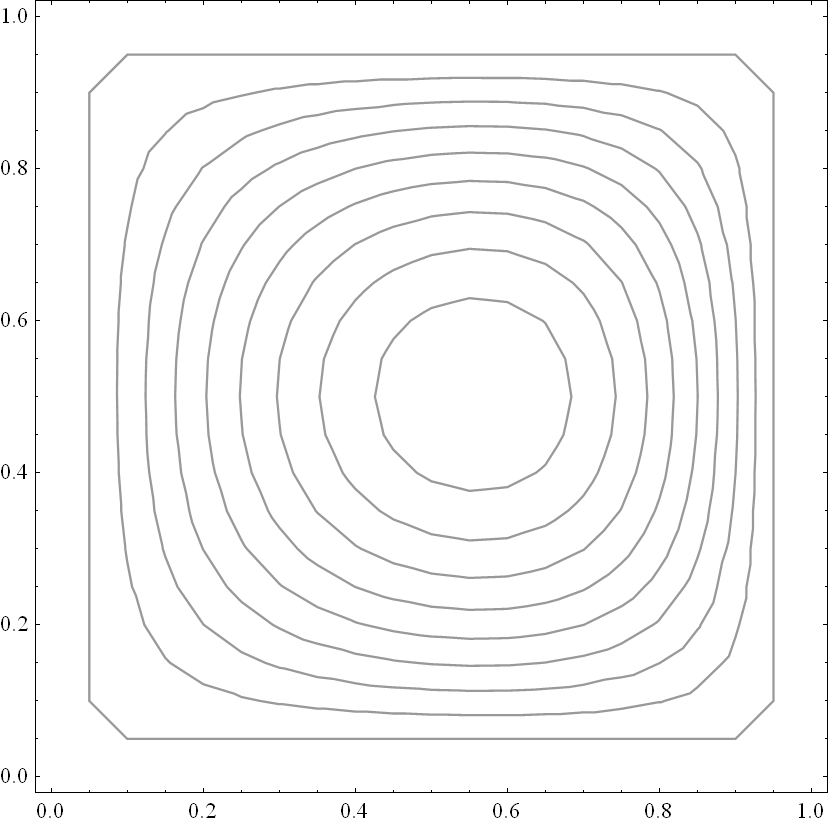
\includegraphics[scale=0.25]{images/psi_100.png}
    \qquad
    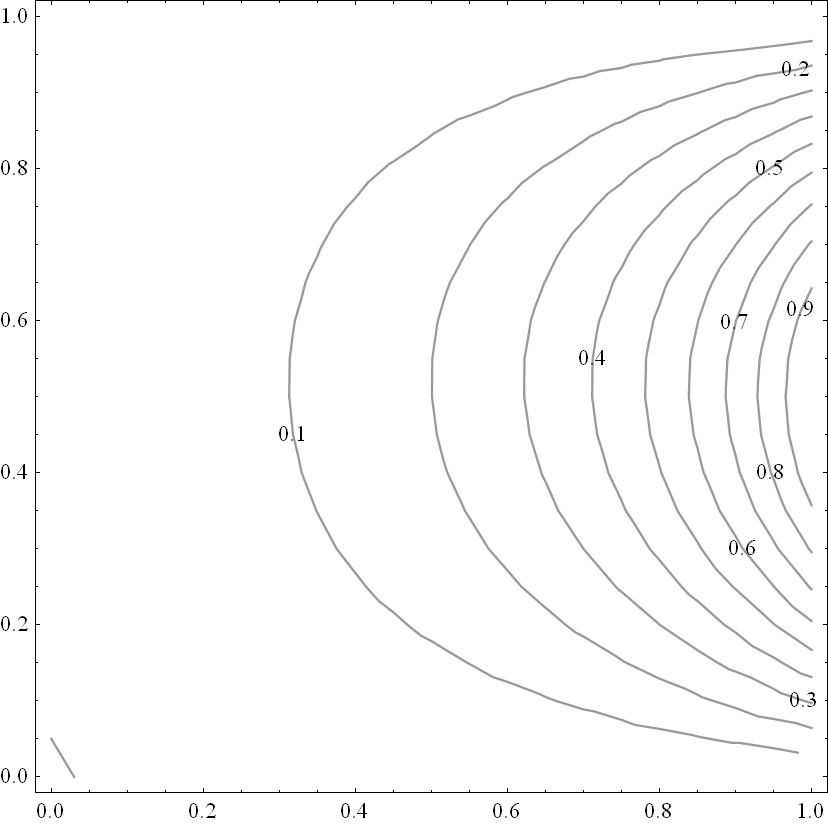
\includegraphics[scale=0.25]{images/t_100.png}

    \bigskip
    Частное решение при $\Pra = 1, \Gra = 10000, N = 20, h = 0.05$:
    \bigskip

    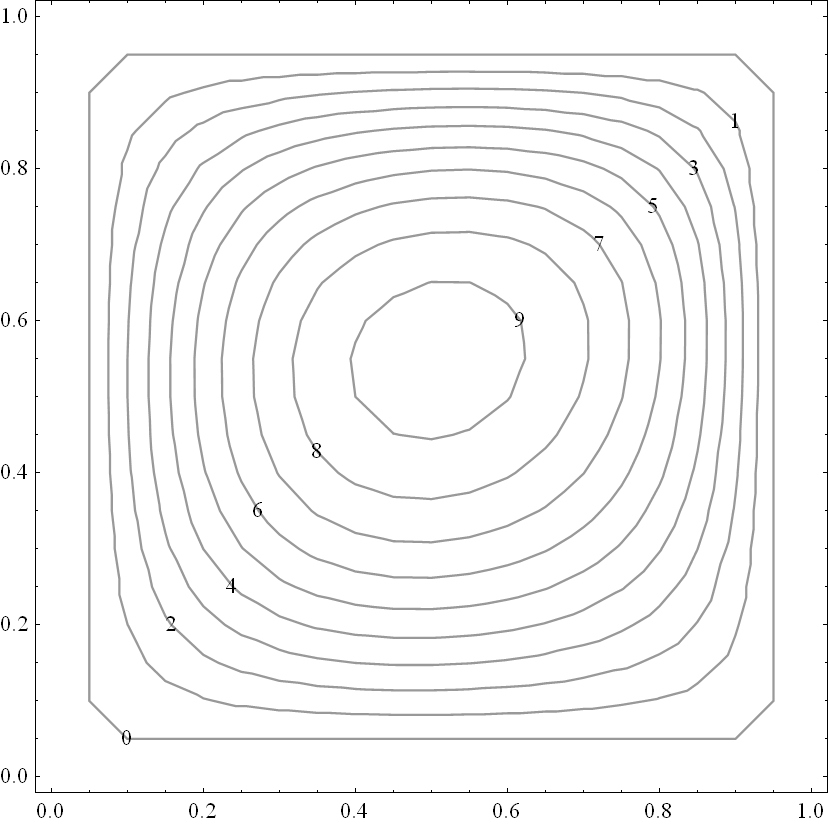
\includegraphics[scale=0.25]{images/psi_10k.png}
    \qquad
    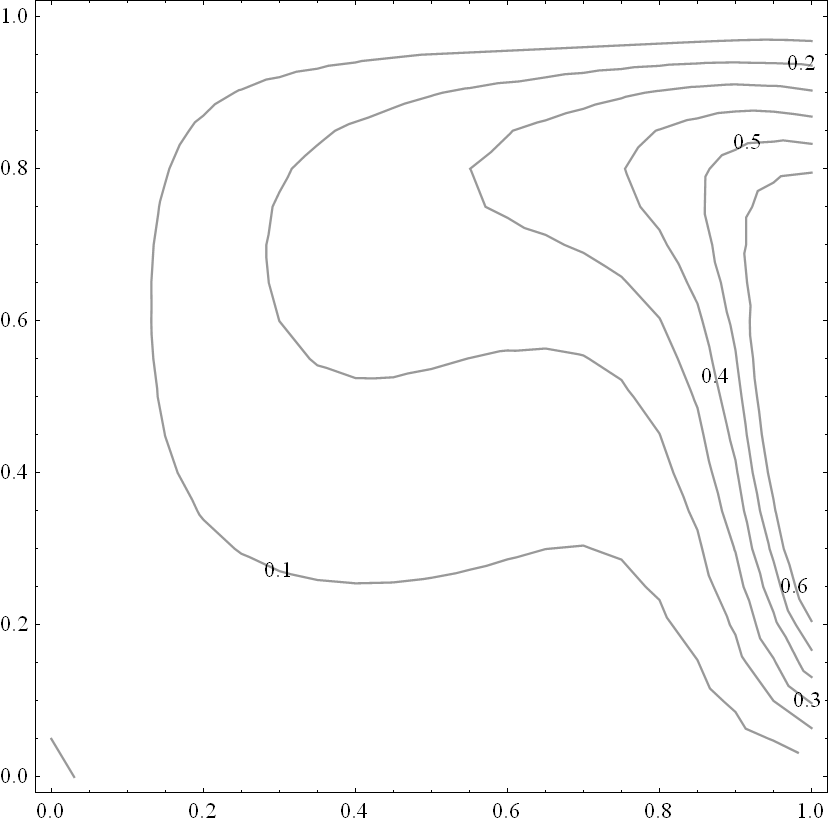
\includegraphics[scale=0.25]{images/t_10k.png}
\end{document}
